\documentclass[11pt]{article}
\usepackage[utf8]{inputenc}
\usepackage{amsmath}
\usepackage{titlesec}
\usepackage{titling}
\usepackage{geometry}
\usepackage{graphicx}
\usepackage{hyperref}
\usepackage{fancyhdr}
\usepackage{wallpaper}
\usepackage{afterpage} 
\usepackage{pagecolor} 
\usepackage{multirow}
\usepackage{wrapfig}
\usepackage{lipsum} % for dummy text
\usepackage{graphicx}
\usepackage[nottoc]{tocbibind} % Put the bibliography in the ToC
\usepackage{url}
\usepackage[toc,page]{appendix}
\usepackage{mdframed}


% Define colors
\usepackage{xcolor}
\definecolor{myblue}{RGB}{33, 66, 99}
\definecolor{mygray}{RGB}{169, 169, 169}
\definecolor{darkbluegrey}{RGB}{44, 62, 80} 

% Page styling
\pagestyle{fancy}
\fancyhf{}
\renewcommand{\headrulewidth}{0pt}
\renewcommand{\footrulewidth}{0pt}
\fancyfoot[C]{\thepage}
\renewcommand{\familydefault}{\sfdefault}

% Define a command for section headers
\titleformat{\section}
  {\color{myblue}\normalfont\Large\bfseries}
  {\color{myblue}\thesection}{1em}{}

% Define a command for subsection headers
\titleformat{\subsection}
  {\color{myblue}\normalfont\large\bfseries}
  {\color{myblue}\thesubsection}{1em}{}

% Adjust page margins
\geometry{a4paper, margin=1in}

% make references clickable
\hypersetup{
    colorlinks=true,
    linkcolor=blue,
    filecolor=magenta,      
    urlcolor=cyan,
}

\begin{document}

% Change the background color of the first page
\pagecolor{darkbluegrey}
\afterpage{\nopagecolor}

% Add a background image
\ThisCenterWallPaper{0.75}{./image/bi.png}

\begin{titlepage}
  \vspace*{\stretch{1}}
  \begin{center}
    \textcolor{white}{\textbf{\Huge Description of Work}}\\ % changed text color to white
    \vspace{1cm}
    \textcolor{white}{\Large Sound Detection and Classification\\using Spiking Neural Networks} % changed text color to white
    \vspace{3cm}
  \end{center}
  \vspace*{\stretch{2}}
  \begin{center}
    \textcolor{white}{ % changed text color to white
      \textbf{COURREGE Téo}\\
      \textbf{GANDEEL Lo'aï}\\
      \vspace{1cm}
      \Large Date: \today}
  \end{center}
  \vspace*{\stretch{1}}
\end{titlepage}

\newpage

\tableofcontents

\pagebreak

\section{Introduction}

In the constantly evolving landscape of neural network studies, the project outlined in this Description of Work (DoW) proposes to explore the field of spiking neural networks (SNNs). This effort will at term combine both a study and a prospective implementation, with a focus on the emerging field of neuromorphic computing.

The overall goal of this project is to perform a thorough investigation and subsequent implementation of spiking neural networks. SNNs, which are inspired by the neural signaling patterns of the human brain, show promising potential in various applications, especially in real-time processing and pattern recognition.

Before getting into the specifics of our project, let us first give a brief overview of what spiking neural networks are and how they work:

A Spiking Neural Network (or SNN) is a type of artificial neural network that mimics the functionality of biological neural networks. Unlike traditional neural networks (ANNs - Artificial Neural Networks), SNNs incorporate the concept of time into their operating model. The neurons in SNNs generate spikes of activity and communicate through these spikes (like brain neurons stimulating each other with electrical impulses), allowing them to process information in a more complex and potentially more efficient manner.

This type of neural network is theoretically less energy consuming than some ANNs and potentially more efficient in terms of processing power (in practice, it will be necessary to create an adapted hardware architecture to take advantage of this potential). Therefore, it seems that the use of this type of neural network could be a viable solution to a classification processing problem (especially in real time ones).

Our project focuses on a specific problem within the broader domain of audio classification.

We will begin this DoW with a brief introduction of our topic, followed by a detailed presentation of the dataset used and its construction. We will then review the state of the art in SNNs and audio classification. After that, we will present the technical goals of our project and a simple theoretical study of SNNs. Finally, we will present the resources at our disposal to carry out this project, as well as a description of the work to be done. Finally, we will propose a timeline for the project.

\pagebreak

\section{Chosen theme}
\subsection{The SNN}
\subsubsection{Definition}

\begin{wrapfigure}{r}{0.5\textwidth}
  \centering
  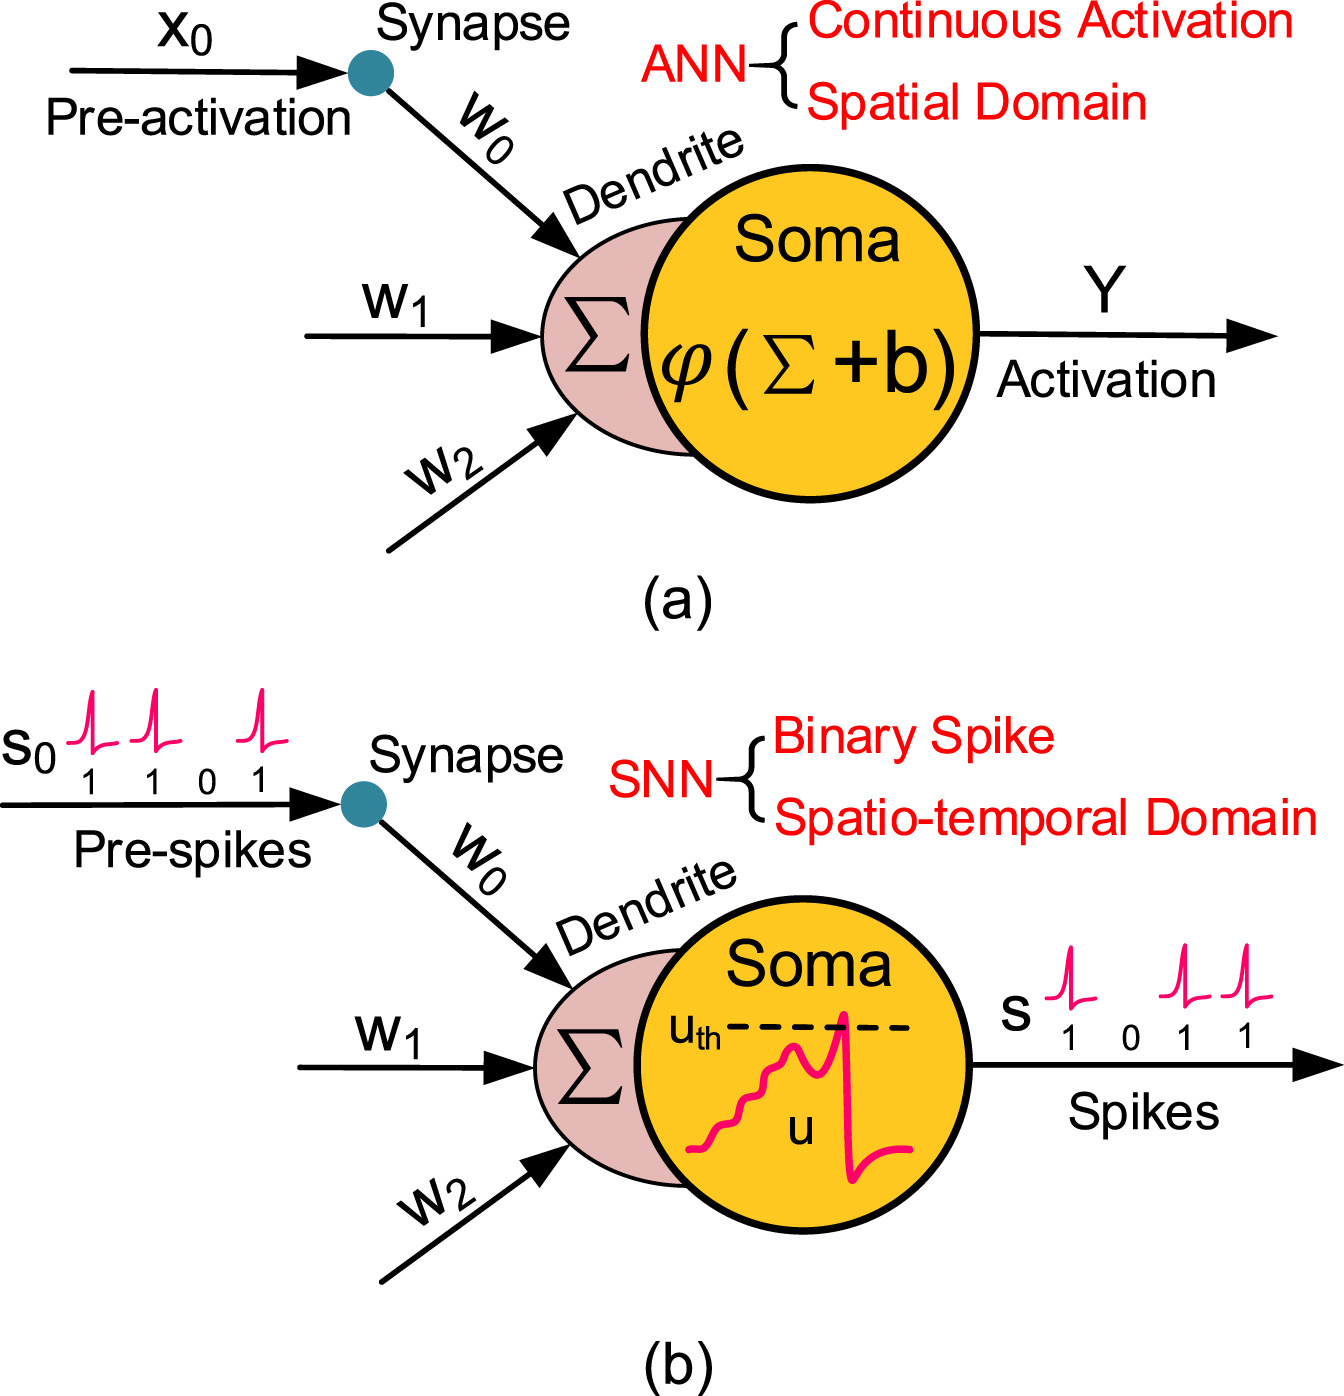
\includegraphics[width=0.48\textwidth,height=0.213\textheight,keepaspectratio]{./image/sums_up.jpg}
  \caption{Difference ANN and SNN model\cite{rething_comparison_ann_snn}}
\end{wrapfigure}


Spiking Neural Network (SNN) is a variant of artificial neural networks that tries to mimic biological neural networks more accurately. More specifically, it tries to copy the way neurons and synapses work. As a result, instead of working with continuously changing time values as ANNs do, SNNs work with discrete events that occur at defined times. SNNs take a set of spike values as input and produce a set of spike values as output.

The spiking behavior of a neuron in an SNN is modeled by a membrane potential equation. For example, in a leaky integrate-and-fire (LIF) neuron model, we have:

\begin{equation}
  \begin{cases}
    \tau \frac{d \: u(t)}{dt} = - [u(t) - u_{r_1}] + \sum_j w_j \sum_{t_j^k \in  S_i^{T_w}} K(t - t_j^k) \\
    \begin{cases}
      s(t) = 1 & u(t) u_{r_2} \text{ if } u(t) \geq u_{th} \\
      s(t) = 0 & \text{otherwise}
    \end{cases}
  \end{cases}
\end{equation}

where $t$ denotes the time step, $\tau$ is a time constant, and $u$ and $s$ are membrane potential and output spike, respectively.
$u_{r_1}$ and $u_{r_2}$ are the resting potential and reset potential, respectively. $w_j$ is the synaptic weight from the $j^{th}$ input neuron, $t_j^k$ is the time when the $k^{th}$ spike of the $j^{th}$ input neuron fires within the integration time window of $T_w$ (a spike sequence of $S_j^{T_w}$ in total), and $K(.)$ is a kernel function describing the time decay effect. $u_{th}$ is the firing threshold that determines whether to fire a spike or not. \cite{rething_comparison_ann_snn}

This model has the advantage of being easier to implement than other kinds of models like the Hodgkin-Huxley model or the Izhikevich model.


\begin{figure}[h]
  \centering
  \begin{minipage}{0.45\textwidth}
    \centering
    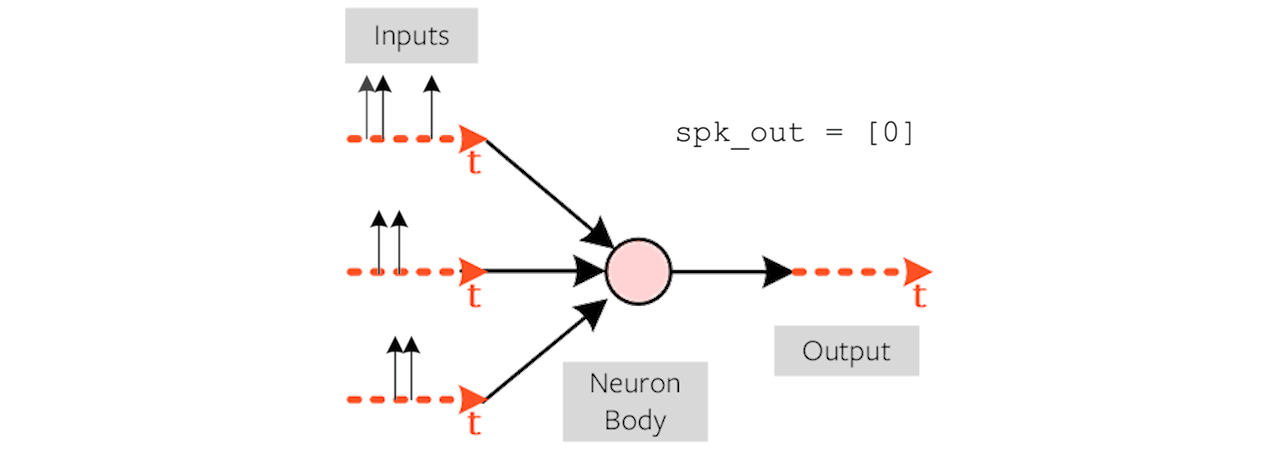
\includegraphics[width=1\textwidth]{image/def1.png}
    \caption{SNN input}
  \end{minipage}\hfill
  \begin{minipage}{0.45\textwidth}
    \centering
    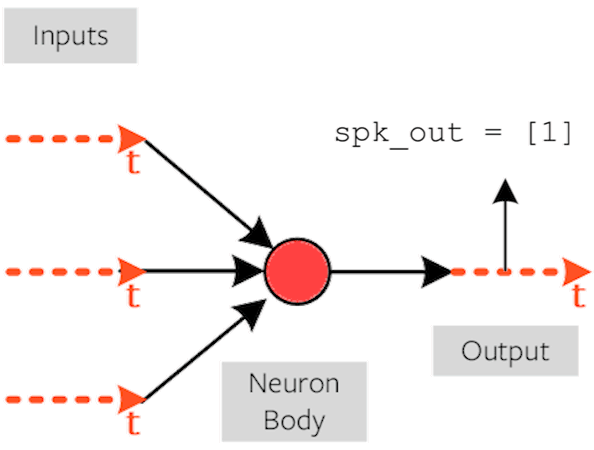
\includegraphics[width=1\textwidth]{image/def2.png}
    \caption{SNN output}
  \end{minipage}
\end{figure}

\pagebreak

\begin{mdframed}[frametitle={Note:}]

  We also found this kind of equation for the membrane potential for a LIF neuron model:

  $$
    \tau \frac{d \: U_j(t)}{dt} = - U_j(t) + \sum_{i=1}^{N} w_{ij} . n_i(t)
  $$

  where, $\tau$ is the leakage time constant, and $n_i(t)$ is the input value of ith neuron, and $w_{ji}$ is a synaptic weight (conductance) between neuron $i$ and $j$. Membrane potential $U(t)$ increases whenever post-synaptic spike is generated by input spikes and it will decay spontaneously with time constant, $\tau$. When the potential crosses over the pre-defined threshold level, it fires a post-synaptic spike and $U(t)$ instantaneously relaxes to the resting state and maintains the level for a refractory time, tref. without responding to any received signals.\cite{memristor_synapses}

  Here, \(V(t)\) is the membrane potential, \(W_i\) is the synaptic weight, and \(\delta(t - t_i)\) is the Dirac delta function representing the occurrence of a spike at time \(t_i\).

  The output spikes \(Y\) can be obtained based on a threshold \( \theta \):
  $$
    Y(t) =
    \begin{cases}
      1 & \text{if } V(t) \geq \theta \\
      0 & \text{otherwise}
    \end{cases}
  $$

\end{mdframed}

\subsubsection{Advantages / Disadvantages}

SNNs, when well designed, should provide the following benefits

\begin{itemize}
  \item Energy efficiency: SNNs are highly energy efficient because they only consume energy when a spike is generated, unlike "classical" neural networks which consume energy continuously. This makes them ideal for low-power embedded devices.

  \item Event-driven processing: While ANNs typically operate at a fixed time interval, SNNs only process information when there is an input spike. This makes them highly efficient at processing information in an event-driven environment, such as processing visual or audio data.

  \item Temporal coding: SNNs are able to process information based on the timing of spikes, allowing them to encode temporal information and be temporally accurate. This is particularly useful for tasks that require the processing of sequential data, such as speech or gesture recognition.

  \item Robustness to noise: SNNs are inherently robust to noise and can effectively filter out irrelevant information. This makes them useful in environments where noise is a common problem, in our case, it may be a case of improperly recorded audio.

  \item Neuroplasticity: SNNs are able to adapt to new inputs and change their behavior over time, much like the brain. This allows them to learn and adapt to new tasks and environments, making them highly versatile.

\end{itemize}


Disadvantages:

\begin{itemize}
  \item SNNs are difficult to train, mainly due to backpropagation issues, which are caused by the discrete, temporal nature of spikes. Backpropagation in time (BPTT) is the typical method used, but it suffers from issues such as the temporal credit assignment problem (the determination of which past events or actions contributed most significantly to the current outcome or state)

        Moreover, the memory and the compute cost can be calculated by:
        \begin{equation}
          \begin{cases}
            \text{ANN:} & M = M_w + M_a       \\
            \text{SNN:} & M = M_w + M_p + M_s
          \end{cases}
        \end{equation}
        Where $M_w$, $M_a$, $M_p$ and $M_s$ denote the memory cost for weights, activations, membrane potentials, and spikes, respectively. Compared to the static values of $M_w$, $M_a$, and $M_p$ that are determined by the network structure, $M_s$ is dynamically determined by the maximum number of spike events at a certain time step.\cite{rething_comparison_ann_snn}

        \begin{equation}
          \begin{cases}
            \text{ANN:} & C = C_{mult} + C_{add} \\
            \text{SNN:} & C = C_{add}
          \end{cases}
        \end{equation}
        where $C_{mult}$ and $C_{add}$ are the compute cost for multiplications and additions, respectively (note that elements such as the activation function in ANNs and the membrane potential update and firing activity in SNNs are ignored) \cite{rething_comparison_ann_snn}
  \item There is currently no learning algorithm designed specifically for this task, SNNs lacks the "maturity" of more classic neural networks.

  \item Building a small SNN is impractical. Indeed, we need a sufficient number of neurons to retrieve useful informations.

  \item We will try to highlight these specificities during our project
\end{itemize}

\subsubsection{snnTorch}
We will work primarily in Python and use the \hyperref[item:snntorch-lib]{snnTorch} library to work on SNNs. snnTorch is a Python package for performing gradient-based learning with spiking neural networks. snnTorch is built on top of Pytorch and takes advantage of its GPU-accelerated tensor computation. Predefined spiking neuron models are integrated into the PyTorch framework and can be treated as recurrent activation units.


\subsection{Neural networks applied to audio classification}
\subsubsection{Definition}
Audio classification is a machine learning and signal processing task that involves categorizing or labeling audio data into different predefined classes or categories. The goal is to automatically assign a label to an audio segment based on its content or characteristics. This can be useful in several applications:

\begin{itemize}
  \item Speech recognition: Identifying spoken words or phrases in audio recordings.
  \item Music genre classification: Classify music into different genres, such as rock, pop, jazz, etc.
  \item Environmental Sound Analysis: Detect and classify environmental sounds such as sirens, footsteps, or car engines.
  \item Anomaly Detection: Identify unusual or unexpected sounds in a given context.
\end{itemize}

\subsubsection{How it works}

The process of audio classification is relatively similar to image classification and typically involves the following steps

\begin{enumerate}
  \item Data collection: Collecting a dataset of audio samples, each labeled with its corresponding class or category.

  \item Feature extraction: Transforming the raw sound data into a set of relevant features that can be used to represent the content of the audio. Common features include spectrogram representations, Mel Frequency Cepstral Coefficient, and other time or frequency domain features.

  \item Model training: Use machine learning algorithms or deep learning architectures to train a model on the extracted features and their corresponding labels.

  \item Validation and testing: Evaluate the performance of the trained model on a separate set of data that it has not seen before. This helps evaluate the model's ability to generalize to new, unseen examples.
\end{enumerate}

\subsection{Relevance of this choice}
\subsubsection{Defining the project's pros and cons}
Pros :
\begin{itemize}
  \item SNN's can be effective for detecting and recognizing different types of audio (especially on embedded devices).
  \item The comparison between SNN and other types of neural networks will be particularly important to us, and we will try to show what can be the strengths and drawbacks of SNNs compared to other networks.
\end{itemize}

Cons:

\begin{itemize}
  \item SNNs can be difficult to understand sometimes, we will need to study the snnTorch library.
  \item Training SNNs is more difficult, and we need to find the most efficient encodings/decodings, training method, and parameters.
\end{itemize}

\subsubsection{Cases of use to define the relevance of the project}
Our final goal is primarily to compare the efficiency and energy use of SNNs compared to others networks (CNNs, RNNs, LSTMs...) in audio classification, and to evaluate if SNNs are a good solution in our case.


\section{Data used}
\subsection{Choosing the type of training data}

When we first read the survey about $SNNs^{\cite{snn_survey}}$, it was understood that training this type of model would be more difficult than some ANNs due to the temporal dynamics involved in SNNs. This made us want to work on a type of data that would be less computationally or resource intensive than videos (so that we could store and train our models on many of them). This type of data also has the advantage of being more adaptable to pre-recorded and real-time processing.
\subsection{Feasibility}

In our case, we decided to apply our analysis to the \hyperref[item:google-audioset]{Google AudioSet} database, which contains a large number of audio samples classified into different categories.
The structure of this dataset is as follows: each audio sample is associated with a label, and each label is associated with a set of audio samples. In practice, this dataset is composed of '.csv' files that contain one or more labels, a timecode (10 seconds of duration), and a part of an url that would help us find an associated Youtube video. This gave us 2 problems: a copyright problem and the fact of extracting the data and formatting it in a way that would be usable for our project.

\subsubsection{Copyright}

According to \hyperref[item:google-audioset]{the AudioSet website} (download page): \begin{quote}

  The dataset is made available by Google Inc. under a Creative Commons Attribution 4.0 International (CC BY 4.0) license, while the ontology is available under a Creative Commons Attribution-ShareAlike 4.0 International (CC BY-SA 4.0) license.\end{quote}


\subsubsection{Data collection/extraction}

Fortunately for us, we found \hyperref[item:google-audioset-reformatted]{some GitHub repositories} whose code aims to download, format, and crop the various sound files so that it "unifies the formats of the datasets so that it is possible to analyze them in the same pipelines". The given script also included a parallelization of the calculation.

After some slight modifications we were able to check the impact on memory resources, for example for \href{https://www.youtube.com/watch?v=dQw4w9WgXcQ}{this youtube video} we get

\begin{itemize}
  \item Resource usage (RAM, GPU, CPU, time)
        \subitem Size of 144p: 2-4 MB (depending on format)
        \subitem Size of the same video as an audio file (wav in best quality): 1-3 MB (depending on the format)
\end{itemize}

Without parallelizing the code we used, we were able to download, format, and trim 6 audio files in about 60 seconds (and our first attempts at parallelizing seemed promising, though there are still bugs to work out). At this pessimistic rate, we think we should be able to download, format and trim about 2000 10-second audio files in about 5-6 hours. By limiting the number of labels to study to about ten, we think we might get some results (to be tested with a pre-trained Pytorch model).

\subsubsection{Uncertainties about data quality}

While lookin up to the data, we found that a lot of these sounds are taken out of context and other sounds are mixed with them (for example, \hyperref{https://www.youtube.com/watch?v=-0CamVQdP_Y}{}{}{this} sample is labeled with as a music sound but a person is talking at the end of the sample). Also, each sample can have one or multiple labels, which can be related to multi-clustering problems.
Another problem we face is the fact that the data is always balanced (there exists a balanced version of the dataset) and that there are some Weak and Strong Label annotations.

Strong labels are precise and indicate the exact start and end times of the event in the audio file whereas the Weak labels, only indicate the presence of a sound event somewhere in the audio file, without specifying the exact time.
\subsection{Open to other databases}

In the case that we use for this classification purpose is not sufficient (for example when collecting all the data related to a unique label), We might try to complete it with other open-source label databases such as \href{https://www.freesound.org/}{Freesound} or \href{https://www.kaggle.com/}{Kaggle}.

\pagebreak

\section{State of the art}

While searching for existing work on the topic, we found that there are already some studies on the subject of audio classification using SNNs. We will present a couple of them here.
\subsection{ANNs Used for Audio Classification}

First of all, we made some researches to find some existing ANNs made for audio classification for comparison with the model we plan to build.
We found the following models:
\begin{itemize}
  \item A VGG model already trained of the Google AudioSet dataset \hyperref[item:vgg-audioset_audioset]{(GitHub)}.
  \item Rearanged Resnet, inception, densenet pretrained models \hyperref[rethink-CNN-for-audio-classification]{(GitHub and research paper)}
  \item An audio classifier that uses LSTM (made in class of Deep Learning): \hyperref[item:lstm-audio-classification]{(Google Colab)}
  \item others: \href{https://medium.com/@aakash__/classifying-audio-using-pytorch-84861f3505ea}{1} \href{https://learn.microsoft.com/en-us/training/modules/intro-audio-classification-pytorch/4-speech-model}{2} \href{https://github.com/yeyupiaoling/AudioClassification-Pytorch}{3} \href{https://github.com/IBM/audioset-classification}{4}
\end{itemize}

\subsection{SNNs Used for Audio Classification}

Secondly, we made some researches to find some existing SNNs made for audio classification, again, for comparison with the model we plan to build.
We found the following models:
\begin{itemize}
  \item A spiking convolutional neural network (SCNN) for audio classification \hyperref[item:SCNN-audio-classification]{(GitHub)}.
  \item A multi-layer SNN for audio classification using SpiNNaker \hyperref[item:spinnaker-audio-classification]{(GitHub)}.
  \item Shadow training ("conversion" of an ANN to an SNN) \hyperref[item:shadow-training]{(GitHub and research paper)}.
  \item Spiking used for image classification \hyperref[item:stereospike]{(GitHub and doc)}.
  \item SNN simulators : \href{item:bindsNET_snntorch-lib}{BindsNET} and \href{item:nest_snntorch-lib}{NEST}
\end{itemize}

The results we may get from the aforementioned networks may serve as a basis of comparison for some of them.


\section{Technical objectives of the project}
\subsection{Technical objectives achievable with pre-existing ANNs}

We should find pre-trained ANNs that can achieve good accuracy with AudioSet.

\subsection{Technical objectives with data}

In its raw form, sound is an analog signal that must be converted to digital. Analog signals are continuous waves. An analog wave has a discrete value at each given point in time. It's impossible to convert every value to a digital representation because there are infinite points in a continuous wave. We will have to convert the audio signal to digital through sampling and quantization. In our case, since we are extracting the audio from YouTube, the conversion to a digital signal step has already been done.

After the conversion, the next step will be to extract useful features from the audio. Some critical features used for audio classification with ML are

\begin{itemize}

  \item Time domain features are extracted directly from the raw audio (waveform). Examples include amplitude envelope and root mean square energy. Time domain features are not sufficient to represent the sound because they do not contain frequency information.

  \item Frequency-domain features are also called the spectrum. Examples include band energy ratio, spectral flux, and spectral bandwidth. These features lack time representation. They are extracted from a time domain representation using the Fourier transform. The Fourier transform converts a waveform from a function of time to a function of frequency.

  \item Time and frequency domain features extract a spectrogram from the waveform using a short-time Fourier transform, such as Spectrogram or Mel Spectrogram. The spectrogram shows both the frequency and time domains. Spectrograms represent frequency linearly, but humans perceive sound logarithmically. This means that humans can tell the difference between lower frequencies, such as 500-100 Hertz (Hz), but have a harder time distinguishing between sounds at higher frequencies, such as 10,000 Hz to 15,000 Hz. This difficulty is why the Mel scale was introduced. A Mel spectrogram is a spectrogram on the Mel scale that measures how different pitches sound to the listener. It maps pitches that sound equidistant to the listener.
\end{itemize}


\begin{figure}[h]
  \centering
  \begin{minipage}{1\textwidth}
    \centering
    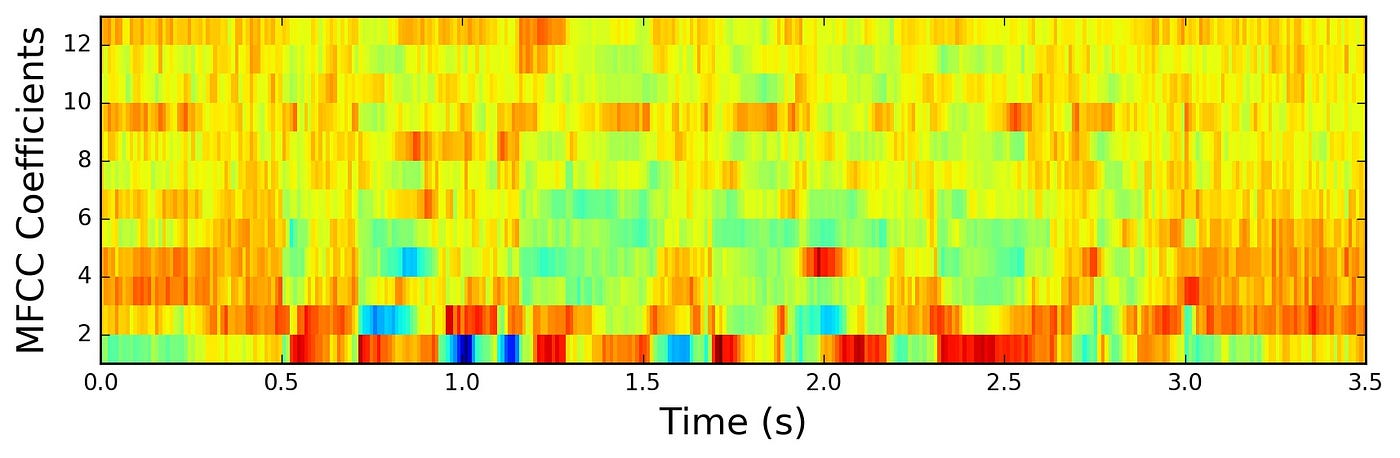
\includegraphics[width=1\textwidth]{image/spectro.jpg}
    \caption{Mel Spectrogram}
  \end{minipage}\hfill
\end{figure}

\subsection{Technical objectives with SNNs}

We need to either find a pre-trainedmodel our create it ourselves. We found a framework for the creation a SNN for robust sound classification.${\cite{model_framework}}$


\subsection{Feasibility}
\subsubsection{Describing Uncertainties}
Uncertainties are mostly due to the dynamic nature of audio signals, varying acoustic environments, and the complexity of differentiating between various sound patterns. Additionally, challenges in precisely modeling the temporal aspects of auditory processing and understanding the dynamics of spiking neurons contribute to many uncertainties in the feasibility of the project. Furthermore, training Spiking Neural Networks to achieve good accuracy is difficult due to the inherent non-linearity and sparsity of spikes.

Regarding data uncertainties, dealing with Youtube means that some audio may not be in the right format (a 5s video from which we extract a 10s audio for example), and some may not even be available (users delete their video), which could lead to unbalanced data.


\subsubsection{Finding a Working Model}

Many models for sound classification already exist. In particular, there are several pre-trained deep neural networks for AudioSet, such as YamNet. However, open source SNNs are harder to find, as they are less widely used than other types of neural networks.

\subsubsection{Computation Time Estimation}

Data import and training are the most time-consuming tasks. We don't know yet how long a training will take. For importing audio, we estimate a little over 10 seconds on average for importing a single audio sample without parallelization, we expect to import between 1,000 and 10,000 audio samples.


\section{Theoretical study}
\subsection{Theoretical study of SNN}

There are multiple archetypes of spiking, each model as its specificity, and while it seems interestig to confine ourselves to the LIF (Leaky Fire and Integrate), which seems the more interesting, it may be relevant to analyze some types of models to evaluate their efficiency. ${\cite{firing_comparison}}$

We will need to choose a lot of parameters regarding our neural network, such as the encoding, the type of training.

Neural coding schemes are used to convert input pixels into spikes that are sent to the excitatory neurons. There are four main neural coding schemes: rate coding, time-to-first spike coding, phase coding, and burst coding.${\cite{codings}}$

There are also different ways to train a SNN:
\begin{itemize}
  \item Shadow training: A non-spiking ANN is trained and converted to a SNN by interpreting activations as firing rate or spike time.
  \item Backpropagation using spikes: The SNN is natively trained using error backpropagation, typically through time as in sequential models.
  \item Local learning rules: Weight updates are a function of signals that are spatially and temporally local to the weight, rather than a global signal as in error backpropagation.
\end{itemize}

\pagebreak
\section{Matching with available resources}
\subsection{Work time}


\begin{center}
  \begin{tabular}{ |p{5cm}||p{3cm}|p{3cm}| }
    \hline
    \multicolumn{3}{|c|}{Schedule}                                                     \\
    \hline
    Task                                          & Duration             & When        \\
    \hline
    \textbf{Data collection/extraction}           &                      &             \\
    From csv/Youtube to mp3                       & 2-3 days             & 22/11-24/11 \\
                                                  &                      &             \\
    \textbf{Data preprocessing}                   &                      &             \\
    cleaning/enhancement/                         &                      &             \\
    augmentation                                  & 3-4 days             & 24/11-28/11 \\
                                                  &                      &             \\
    \textbf{Models implementation}                &                      &             \\
    understanding snnTorch basics                 & 2 days               & 22/11-24/11 \\
                                                  &                      &             \\
    finding pretrained/creating and tuning models & 4-5 days             & 26/11-01/12 \\
                                                  &                      &             \\
    \textbf{Training/tuning}                      &                      &             \\
    training                                      & multiple weeks       &             \\
                                                  &                      &             \\
    extracting/synthetizing info                  & multiple weeks       &             \\
                                                  &                      &             \\
    \textbf{Working on the DOWs and presentation} &                      &             \\
    DOWs writing: continous work                  & 2 hours x 2 per week &             \\
                                                  &                      &             \\
    slides for oral presentation                  & 2-3 days             & 27/11-29/11 \\
    \hline
  \end{tabular}
\end{center}



\subsection{Computer resources}

We will work with the following:
\begin{itemize}
  \item Hardwares: 2 laptops
  \item Softwares: Google Colab (primarily), Kaggle
\end{itemize}

\subsection{Human resources}

We will work in parallel most of the time, each one focusing on a different aspect to gain time when it is possible.

\pagebreak

\section{Appendix}

\subsection{Data}

\subsubsection*{Data Set used for the project}

\begin{itemize}
  \item Google AudioSet : \url{https://research.google.com/audioset/}
        \label{item:google-audioset}
\end{itemize}

\subsection{Existing models}

\begin{itemize}
  \item Sparsity through Spiking Convolutional Neural Network (SCNN) for Audio Classification at the Edge : \url{https://github.com/CongSheng/SpikingConvNN-AudioClassification/tree/main}
        \label{item:SCNN-audio-classification}
  \item Multilayer Spiking Neural Network for audio samples classification using SpiNNaker : \url{https://github.com/jpdominguez/Multilayer-SNN-for-audio-samples-classification-using-SpiNNaker}
        \label{item:spinnaker-audio-classification}

  \item StereoSpike: Depth Learning With a Spiking Neural Network for image classification (CNN) : \url{https://github.com/urancon/stereospike} - \url{https://ieeexplore.ieee.org/document/9969606} \label{item:stereospike}

  \item Spiking Neural Networks Trained via Proxy (shadow training): \url{https://ieeexplore.ieee.org/document/9810220} \label{item:shadow-training}

  \item VGG model trained on Google's AudioSet dataset : \url{https://github.com/MaryamEbr/Audio-Classification-with-AudioSet-and-VGGish/tree/main} \label{item:vgg-audioset_audioset} - \url{https://research.google/pubs/pub45611/}

  \item  Rethink CNNs for Audio Classification : \url{https://github.com/kamalesh0406/Audio-Classification/tree/master} - \url{https://arxiv.org/abs/2007.11154} \label{rethink-CNN-for-audio-classification}

  \item An LSTM model for audio classification we made in class of Deep Learning : \url{https://colab.research.google.com/drive/1kJ4hFfh3J13_nrtCMRrPoE_eIl5xUQWC?usp=sharing} \label{item:lstm-audio-classification}

  \item BindsNET, a Python package for training and simulating spiking neural networks : \url{https://github.com/BindsNET/bindsnet} \label{item:bindsNET_snntorch-lib}

  \item NEST, a simulator for spiking neural network models that focuses on the dynamics, size and structure of neural systems rather than on the exact morphology of individual neurons : \url{https://www.nest-simulator.org/} \label{item:nest_snntorch-lib}

\end{itemize}

\subsection{Code}

\begin{itemize}
  \item A collection of scripts to analyze, prepare for and download Google's Audioset : \url{https://github.com/bakhtos/GoogleAudioSetScripts}
        \label{item:google-audioset-reformatted}

  \item SNNtTorch, a Python package for performing gradient-based learning with spiking neural networks : \url{https://snntorch.readthedocs.io/en/latest/} \label{item:snntorch-lib}
\end{itemize}

\pagebreak

% Bibliography
\bibliographystyle{siam}
\bibliography{ref}

\end{document}
